\subsection{Design af Lineær bevægelse i x-, y- og z-retningen} \label{Design af Lineær bevægelse i x-, y- og z-retningen}

Det er valgt at bevæge de to akser seperat, hvilket sikrer at det ønskede arbejdesområde kan tilgås præcist. Arbejdsområdets ene side er længere end den anden, og afstanden har indflydelse på udbøjningen. Det vælges derfor at doserings mekanismen monteres på den korte akse, y-aksen, dette er gjort for at minimere udbøjningen, som det ses i afsnit \ref{Præcisions beregninger}.

Som tidligere beskrevet bevæges y-aksen og hovedet med ledeskruer på $\diameter\SI{10}{mm}$, både x og y vognen glider på to følgestænger, placeret horisontal på hver side af ledeskruen. Hver ledeskrue drives af en NEMA 14 motor, som det ses på figur \ref{fig:xyz akse med navne}. Følgestængerne bære vægten af henholdsvis x-vognen og y-vognen, gennem glidelejre for at minimere friktion. I den modsatte side af motoren er ledeskruen drejet rund og monteret i et kugleleje.


\begin{figure}[H]
    \centering
    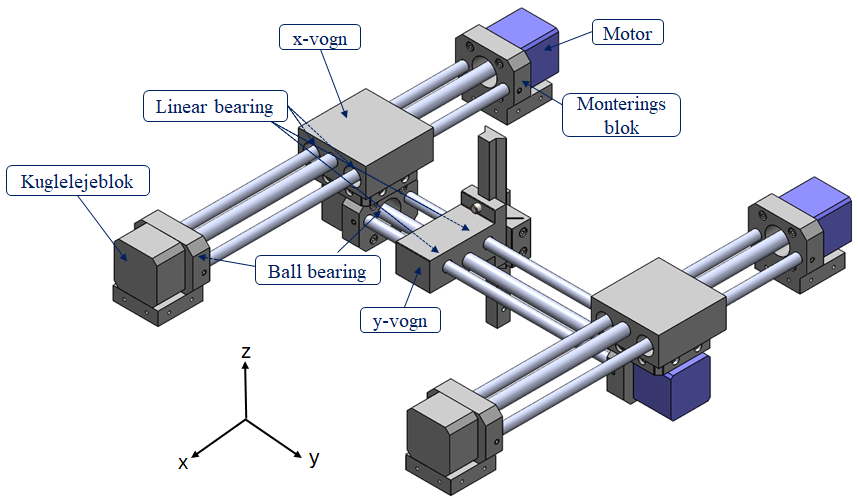
\includegraphics[width=0.8\linewidth]{Sections/6 Detaljeløsning/Media/x,y,z akse med tekst.png}
    \caption{x-, y- og z-aksen med navne}
    \label{fig:xyz akse med navne}
\end{figure} \plainbreak{-0.5}
 
Det er valgt, at y-aksen er fastspændt under x-aksen, så der kan påsættes prikker på emner under \(\SI{50}{mm}\), med den valgte justering af z-aksen. Robotten skal kun håndtere objekter med plane flader, hvorfra det ikke er nødvendigt, at justere z-aksen under processen. Det vælges derfor, at z-aksen justeres manuelt inden robotten startes. Dette gøres med en svanehalemekanisme på y-vognen, som ses i figur \ref{fig:z-akse justering}.

\begin{figure}[H]
    \centering
    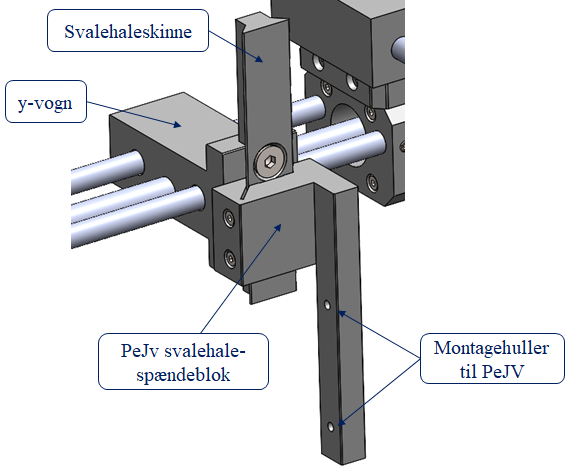
\includegraphics[width=0.6\linewidth]{Sections/6 Detaljeløsning/Media/z-akse med tekst.png}
    \caption{y-vogn med svalehaleblok og svalehale skinne, der bruges til justering af z-aksen. Jet valve DV-6210 monteres på svalehaleskinnen med to M4 bolte i montagehullerne.}
    \label{fig:z-akse justering}
\end{figure} \plainbreak{-0.5}

Her monteres Jet Valve DV-6210 med to M4 bolte i montagehullerne. Svalehaleblokken sættes på y-vognen, hvorefter svalehaleskinnen frit kan bevæges fra bundpladen \(\SI{60}{mm}\) over bundpladen. Alle komponenterne til den lineære bevægelse, der er designet til løsningen, produceres i Aluminium EN AW-6082 T6.

Aluminium EN AW-6082 T6 er et let metal med en densitet på cirka \(\SI{2700}{kg/m^3}\) og et E-modul omkring \SI{71}{GPa}. Aluminiumet tilbyder et gunstigt forhold mellem vægt og stivhed, hvilket gør det velegnet til strukturer, hvor lav masse og tilstrækkelig mekanisk styrke er væsentlige krav. Materialets flydespænding er \SI{255}{MPa}, og dets trækstyrke spænder fra \SI{300}{MPa} til \SI{340}{MPa}. EN AW-6082 T6 har desuden gode bearbejdningsegenskaber, idet det let kan fræses, bores og svejses. En yderligere fordel er dets naturlige korrosionsbestandighed, hvilket reducerer behovet for omfattende overfladebehandling i mange anvendelser. Aluminium er samtidig relativt økonomisk tilgængeligt med en gennemsnitlig pris på omkring 244 DKK pr. kg \parencite{Aluminiumplade}. Ulempen ved aluminium er dog, at materialet i visse tilfælde kan have begrænset modstandskraft over for høje punktbelastninger, hvilket kan føre til lokal plastisk deformation, hvis konstruktionen ikke dimensioneres tilstrækkeligt. \parencite{Hesse2011AluminiumSheets}.


%Da der arbejdes med emner der har en ens højde langs hele emnet, betyder det at under processen behøver der ikke sker regulering i z-aksen. Det er derved blevet valgt at bevægelsen på z-aksen, sker manuelt inden processen starter. 

%De to resterende akser udspænder det planen som der skal kunne sættes prikker. 

%Bevægelsen i xy-planet kommer derved fra to ledskruer på x-aksen og en ledeskrue på y-aksen. Ledeskruerne på x-aksen driver hver deres vogn, som hvorpå y-aksens ledskrue er monteret i den ene ende og monteringsblok i den anden. x-akse ledeskrurerne ænrdre altså placering af ledeskruen for y-aksen, og y-akse ledeskruen ændre placering af PeJV'en.